\section{Experiment and Analysis}
\begin{table*}[t]
\centering
\caption{Comparisons with state-of-the-art NAS and NAD methods. NAS is limited by the expert-defined search space, \ie NAS-Bench-201, while NAD enables the exploration of entirely new architectures beyond the search space. We compare with $\diamondsuit$ methods with parameter sharing, $\heartsuit$ methods without parameter sharing, $\bigstar$ LLM-based methods. We report the mean validation and test accuracies for 5 three runs.
}
\label{tab:nasbench}
\scalebox{0.9}{\begin{tabular}{c|l|c|cc|cc|cc}
\toprule
 & \multirow{2}{*}{Method} & Search & \multicolumn{2}{c|}{CIFAR-10} & \multicolumn{2}{c|}{CIFAR-100} & \multicolumn{2}{c}{ImageNet16-120} \\
 & &  (archs) & validation & test & validation & test & validation & test \\ \midrule
\parbox{2.5mm}{\multirow{16}{*}{\rotatebox[origin=c]{90}{\textbf{NAS}}}} 
 & $\diamondsuit$ ENAS~\cite{pham2018efficient} & - & 37.51±3.19 & 53.89±0.58 & 13.37±2.35 & 13.96±2.33 & 15.06±1.95 & 14.84±2.10 \\
 & $\diamondsuit$ DARTS \cite{liu2018darts}  & - & 39.77±0.00 &  54.30±0.00 &  38.57±0.00 & 15.61±0.00 &  18.87±0.00 &  16.32±0.00 \\
 & $\diamondsuit$ SETN~\cite{dong2019one} & - & 84.04±0.28 & 87.64±0.00 & 58.86±0.06 & 59.05±0.24 & 33.06±0.02 & 32.52±0.21  \\
 & $\diamondsuit$ DSNAS \cite{hu2020dsnas}  & - & 89.66±0.29 & 93.08±0.13 &  30.87±16.40 & 31.01±16.38 & 40.61±0.09 & 41.07±0.09 \\
 & $\diamondsuit$ PC-DARTS \cite{xu2019pc} & -  & 89.96±0.15 & 93.41±0.30 & 67.12±0.39 & 67.48±0.89 & 40.83±0.08 & 41.31±0.22 \\
 & $\diamondsuit$ SNAS \cite{xie2018snas} & - & 90.10±1.04 & 92.77±0.83 & 69.69±2.39 & 69.34±1.98 & 42.84±1.79 & 43.16±2.64 \\ 
 & $\diamondsuit$ iDARTS \cite{zhang2021idarts} & - & 89.86±0.60 & 93.58±0.32 &  70.57±0.24 & 70.83±0.48 &  40.38±0.59 & 40.89±0.68 \\
 & $\diamondsuit$ GDAS \cite{dong2019searching} & - & 89.89±0.08 & 93.61±0.09 & 71.34±0.04 & 70.70±0.30 & 41.59±1.33 &  41.71±0.98  \\
 & $\diamondsuit$ DRNAS \cite{chen2020drnas} & - & {91.55±0.00} & 94.36±0.00  &  73.49±0.00 & 73.51±0.00 & 46.37±0.00 & 46.34±0.00  \\
 & $\diamondsuit$ $\beta$-DARTS \cite{ye2022b} & -  & {91.55±0.00} & 94.36±0.00  & 73.49±0.00 & 73.51±0.00 & 46.37±0.00 & 46.34±0.00  \\
 & $\diamondsuit$ $\Lambda$-DARTS \cite{movahedi2022lambda} & - & {91.55±0.00} & 94.36±0.00  &  73.49±0.00 & 73.51±0.00 & 46.37±0.00 & 46.34±0.00  \\ 
 & $\heartsuit$ REA~\cite{real2019regularized} & 500 &91.19±0.31 & 93.92±0.30 & 71.81±1.12 & 71.84±0.99 & 45.15±0.89 & 45.54±1.03 \\
 & $\heartsuit$ RS~\cite{bergstra2012random} & 500 & 90.93±0.36  & 93.70±0.36& 70.93±1.09 & 71.04±1.07& 44.45±1.10 & 44.57±1.25 \\
 & $\heartsuit$ REINFORCE~\cite{williams1992simple} & 500 & 91.09±0.37 & 93.85±0.37 & 71.61±1.12 & 71.71±1.09 & 45.05±1.02 & 45.24±1.18 \\
 & $\heartsuit$ BOHB~\cite{falkner2018bohb} & 500 & 90.82±0.53 & 93.61±0.52 & 70.74±1.29 & 70.85±1.28 & 44.26±1.36 & 44.42±1.49 \\
 & $\bigstar$GENIUS~\cite{zheng2023can} & 10 & 91.07±0.20 & 93.79±0.09 & 70.96±0.33 & 70.91±0.72 & 45.29±0.81 & 44.96±1.02 \\ 
 & $\bigstar$LLMatic~\cite{nasir2023llmatic} & 2000 & - & 94.26±0.13 & - & 71.62±1.73 & - & 45.87±0.96 \\
 % \rowcolor{blue!20}
 & \mycc  ~~~~\textit{Optimal} & \mycc  - & \mycc 91.61 & \mycc 94.37 & \mycc 73.49 & \mycc 73.51 & \mycc 46.77 & \mycc 47.31 \\ \midrule
 \parbox{2.5mm}{\multirow{8}{*}{\rotatebox[origin=c]{90}{\textbf{NAD}}}}  
 & $\bigstar$LeMo-NADe-Gemini~\cite{rahman2024lemo} & 30 & 82.94 & 81.76 & 52.12 & 52.96 & 30.34 & 31.02 \\
 & $\bigstar$LeMo-NADe-GPT4~\cite{rahman2024lemo} & 30 & 90.90 & 89.41 & 63.38 & 67.90 & 27.05 & 27.70 \\
\cline{2-9}
 & \multirow{3}{*}{$\bigstar$ NADER (Random)} & 0 & 87.67±2.88 & 90.36±2.94 & 64.89±4.94 & 64.81±5.13 & 36.56±6.60 & 36.51±7.11 \\
 &  & 5 & 90.91±0.46 & 94.20±0.38 & 74.11±0.25 & 74.02±0.33 & 48.73±0.19 & 48.72±0.14 \\
 &  & 10 & 91.16±0.36 & 94.40±0.23 & 74.41±0.34 & 74.51±0.16 & \underline{50.07±0.75} & \underline{49.63±0.80} \\
\cline{2-9}
 & \multirow{4}{*}{$\bigstar$ NADER (ResNet)} & 0 & 90.83 & 93.97 & 70.42 & 70.86 & 44.53 & 43.63 \\
 &  & 5 & 91.17±0.24 & 94.52±0.22 & 73.29±1.86 & 73.12±1.09 & 47.98±0.73 & 47.99±0.38 \\
 &  & 10 & 91.18±0.23 & \underline{94.52±0.22} & \underline{74.71±0.45} & \underline{74.65±0.33} & 48.56±0.83 & 48.61±0.76 \\
 &  & 500 &  \textbf{91.55} & \textbf{94.62} & \textbf{75.72} & \textbf{76.00} & \textbf{50.20} & \textbf{50.52} \\
 \bottomrule
 \end{tabular}}
\end{table*}
\subsection{NAD Benchmark}
To facilitate developing and evaluating LLM-based Neural Architecture Design (NAD), we create a comprehensive benchmark dataset. 
We established five types of basic blocks as our starting points: (1) ResNet base block, (2) ResNet bottleneck block, (3) GoogLeNet block, (4) ConvNeXt block and (5) SE-ResNet block. For each basic block, we used GPT-4o to generate some initial macro-level and micro-level modification suggestions. 
We manually inspected and modified the generated modification suggestions, resulting in 10 high-quality macro-level and 10 micro-level modification suggestions for each basic block. There are $(10+10) \times 5 = 100$ test samples in total.
This allows us to evaluate the system's performance on a diverse set of architectural modifications, ranging from basic blocks to more complex structures inspired by state-of-the-art models. Macro-level modification suggestions don't have definitive answers and are more open-ended, while the micro-level modification suggestions have more specific, ground-truth answers. 
For each pair of basic block and its corresponding modification suggestions, we manually checked and generated ground-truth resulting blocks for reference. It is ensured that the resulting blocks reflect the modification suggestions and were executable.

\textbf{Evaluation Metrics.} To assess the performance of our approach, we use the 100 test samples from the NAD benchmark to evaluate the ability to generate valid and executable architectures that adhere to both macro-level and micro-level modification suggestions.
\begin{itemize}
    \item \textbf{Executability (E):} This metric quantifies the agents’ ability to generate executable code as the percentage of successfully executable modified architectures.
    \item \textbf{Quality (Q):} This metric assesses the ability of agents to generate a neural architecture that meets the modification suggestions, quantified as the percentage of modified architectures that successfully implement the specified modification suggestions among the executable ones.
    \item \textbf{Success Rate (SR):} The success rate is a holistic metric that considers both executability and quality, providing a comprehensive measure of the approach's effectiveness.
    \item \textbf{Number of Tokens (\# Tokens):} This metric represents the cost per execution, with a higher number of generated tokens indicating increased computational expense.
\end{itemize}
\subsection{Comparison with State-of-the-art Models}
\textbf{Experimental Setup.}
We conduct experiments to compare both NAS and NAD methods using the well-known NAS-Bench-201~\cite{dong2020bench} benchmark, covering evaluations on CIFAR10, CIFAR100~\cite{krizhevsky2009learning}, and ImageNet16-120~\cite{chrabaszcz2017downsampled}. The results are demonstrated in Table~\ref{tab:nasbench}. 
Our NADER accepts any network as the initial network. In our experiments, we report the results of utilizing ResNet~\cite{he2016deep} as the initial network and the results of using randomly selected networks from the NAS-Bench-201 search space. We report results for designing 5 and 10 new architectures. Each result reflects the mean and standard deviation from three repeated runs with different random seed.

For NAD, the newly designed architecture can be out of the scope of the search space.
To ensure fairness, (1) we constrain the architectures generated by NADER to have the same macro skeleton with NAS-Bench-201. (2) We constrain the FLOPs and parameter count of NAD methods not to exceed the largest network within the NAS search space: paramerts no more than 1.5M for all datasets, FLOPs no more than 0.2 GFLOPs for CIFAR10 and CIFAR100, and FLOPs no more than 0.05 GFLOPs for ImageNet16-120. (3) Model training adhered strictly to the NAS-Bench-201 settings, maintaining the original train/validation/test splits without altering any hyperparameters.

\textbf{Comparisons with NAS methods.}
NAS methods operate within a predetermined search space, focusing primarily on designing cell blocks for neural architectures. Given five operation choices and four nodes for each cell, the total search space expands to $5^6 = 15625$ candidated cells. We evaluated several prominent NAS algorithms, categorized as follows:
(1) Random search algorithms: random search (RS)~\cite{bergstra2012random} and random search with parameter sharing (RSPS)~\cite{li2020random};
(2) ES methods: REA~\cite{real2019regularized};
(3) RL algorithms: REINFORCE~\cite{williams1992simple} and ENAS~\cite{pham2018efficient};
(4) HPO methods: BOHB~\cite{falkner2018bohb}; 
(5) Differentiable algorithms: DARTS \cite{liu2018darts}, SETN~\cite{dong2019one}, DSNAS \cite{hu2020dsnas}, PC-DARTS \cite{xu2019pc}, SNAS \cite{xie2018snas}, iDARTS \cite{zhang2021idarts}, GDAS \cite{dong2019searching}, DRNAS \cite{chen2020drnas}, $\beta$-DARTS \cite{ye2022b}, $\Lambda$-DARTS;
(6) LLM-based methods: GENIUS~\cite{zheng2023can} and LLMatic~\cite{nasir2023llmatic}. We provide the optimal accuracy for reference (\textit{Optimal}), which is the maximum accuracy that can be achieved in the NAS-bench-201 search space. 
Our findings indicate that the NADER framework is robust; even when initialized with a random network, it can be effectively optimized after just a few iterations. Notably, in nearly all scenarios, NADER consistently designs architectures that surpass the optimal accuracy achievable within the predetermined search space, demonstrating the advantages of NAD over traditional NAS methods.

\textbf{Comparisons with NAD methods.} We also compare NADER against the recent NAD method, LeMo-NADe~\cite{rahman2024lemo}, which employs advanced LLMs like Gemini and GPT4-Turbo to refine neural networks based on expert-generated instructions. While LeMo-NADe shows promise, it still falls short compared to more recent NAS methods in certain respects. Our NADER approach significantly surpasses LeMo-NADe in both effectiveness and efficiency. For instance, with a random base network, NADER achieved 49.63\% accuracy on the ImageNet16-120 test set, compared to LeMo-NADe's 31.02\%. Furthermore, NADER requires only 10 trials—three times fewer than LeMo-NADe. These results highlight the potential of leveraging multi-agent collaboration for both effective and efficient NAD in an open architectural space.

\begin{table}[t]
    \centering
    \caption{Ablation studies of Research Team. Experiments are conducted on CIFAR10, CIFAR100, and ImageNet16-120 datasets. We report the results of neural architecture modifications for 5 iterations and show the mean and standard deviation from three repeated runs with different random seed.
    ``R'' and ``P'' represent Reader and Proposer respectively.
    }
    \label{tab:reader}
    \scalebox{0.61}{
    \begin{tabular}{cc|cc|cc|cc}
    \toprule
    \multirow{2}{*}{R} & \multirow{2}{*}{P}  & \multicolumn{2}{c|}{CIFAR-10} & \multicolumn{2}{c|}{CIFAR-100} & \multicolumn{2}{c}{ImageNet16-120} \\
     & & validation & test & validation & test & validation & test \\ 
    \midrule
    \xmark & \xmark & 90.37±0.65 & 94.01±0.42 & 72.55±0.27 & 72.49±0.40 & 47.12±1.26 & 47.14±1.30 \\
    \xmark & \cmark & 90.73±0.32 & 93.73±0.38 & 73.55±1.26 & 73.45±1.32 & 47.88±0.29 & 47.92±0.34 \\
    \cmark & \xmark & 90.86±0.19 & 91.72±2.52 & 73.67±0.85 & 73.37±0.73 & 47.89±1.16 & 47.91±1.00 \\
    \cmark & \cmark & \textbf{90.91±0.46} & \textbf{94.20±0.38} & \textbf{74.11±0.25} & \textbf{74.02±0.33} & \textbf{48.73±0.19} & \textbf{48.72±0.14} \\
    \bottomrule
    \end{tabular}
    }
\end{table}

\subsection{Ablation Studies}
\textbf{Effect of Reader and Proposer.} 
The Reader agent analyzes recent academic papers on neural architectures and related advances, and proposes key innovations and knowledge that could potentially improve neural network performance. 
Then the Reflector agent retrieves appropriate knowledge for the network to enhance it.
To validate the effectiveness of LLM-empowered Reader and LLM-empowered Proposer, we conducted ablation experiments, and the results are shown in Table ~\ref{tab:reader}.
we built two strong baselines.
When both Reader and Proposer are absent, we adopt a set of expert designed modification suggestions used in LeMo-NADe~\cite{rahman2024lemo} to generate design suggestions.
When only the Proposer is present, we prompts LLM to propose design suggestions based on its own knowledge without accessing to the recent achievements. 
When only the Reader is present, we randomly select knowledge from the knowledge pool as design suggestions.
We observe that both Reader and Proposer are important for improving the performance of NAD, especially on the challenging dataset, \ie ImageNet16-120. 

\begin{table}[t]
    \centering
    \caption{Ablation studies of the Developer Team. Experiments are conducted on our NAD benchmark. ``LIF'' and ``LDE'' mean learning from immediate feedback and learning from design experience respectively.
    }
    \scalebox{0.85}{
    \begin{tabular}{c|ccc|c|cc|c}
    \toprule
    Task & Graph & LIF & LDE & \# Tokens (K) & E & Q & SR \\
    \midrule
    \parbox{2.5mm}{\multirow{4}{*}{\rotatebox[origin=c]{90}{\textbf{Macro}}}}  
    & \xmark & \xmark & \xmark  & 2.23±0.27 & 0.64 & 0.63 & 0.40 \\
    & \cmark & \xmark & \xmark  &  0.58±0.66 & 0.54 & 0.78 & 0.42 \\
    & \cmark & \cmark & \xmark  &  0.73±0.82 & 0.64 & 0.84 & 0.54 \\
    & \cmark & \cmark & \cmark  & \textbf{0.53±0.68} & \textbf{0.78} & \textbf{0.87} & \textbf{0.68} \\
    \midrule
    \parbox{2.5mm}{\multirow{4}{*}{\rotatebox[origin=c]{90}{\textbf{Micro}}}}  
    & \xmark & \xmark & \xmark & 2.10±0.22 & 0.76 & 0.65 & 0.49 \\
    & \cmark & \xmark & \xmark &  0.49±0.63 & 0.62 & 0.97 & 0.60 \\
    & \cmark & \cmark & \xmark & 0.48±0.65 & 0.70 & 0.89 & 0.62 \\
    & \cmark & \cmark & \cmark & \textbf{0.31±0.45} & \textbf{0.92} & \textbf{0.96} & \textbf{0.88} \\
    \bottomrule
    \end{tabular}
    }
    \label{tab:develop_team}
\end{table}

\textbf{Effect of Graph-based Neural Architecture Representation.} We compare the graph-based neural architecture representation with the code-generation baseline. Specifically, we carefully design the prompts to prompt the LLM to directly generate codes for modifying the neural network architecture. From the experiments, we find that while existing LLMs demonstrate impressive capabilities in generating executable program codes (64\% executability), the quality is relatively low (63\% quality score). By adopting the graph representation, the LLMs can focus more on designing network architecture without distracted by the code style and formatting. In addition, the graph-based representation is more compact, resulting in fewer required tokens. 


\textbf{Effect of Learning from Immediate Feedback (LIF).} 
The Reflector agent plays a crucial role in improving the executability and the quality of the modified network architecture. Adding LIF improves the executability from 0.54 to 0.64, while improving the quality score from 0.78 to 0.84.  

\textbf{Effect of Learning from Design Experience (LDE).}
The integration of learning from design experience significantly enhances the performance of NAD, in terms of both the executability and the quality, resulting in improved success rate.
For micro-level modifications, the code execution rate of the generated neural network reached 92\% and the success rate is significantly improved from 0.62 to 0.88.

\subsection{Large-scale NAD Experiment}
\begin{figure}[t]
    \centering
    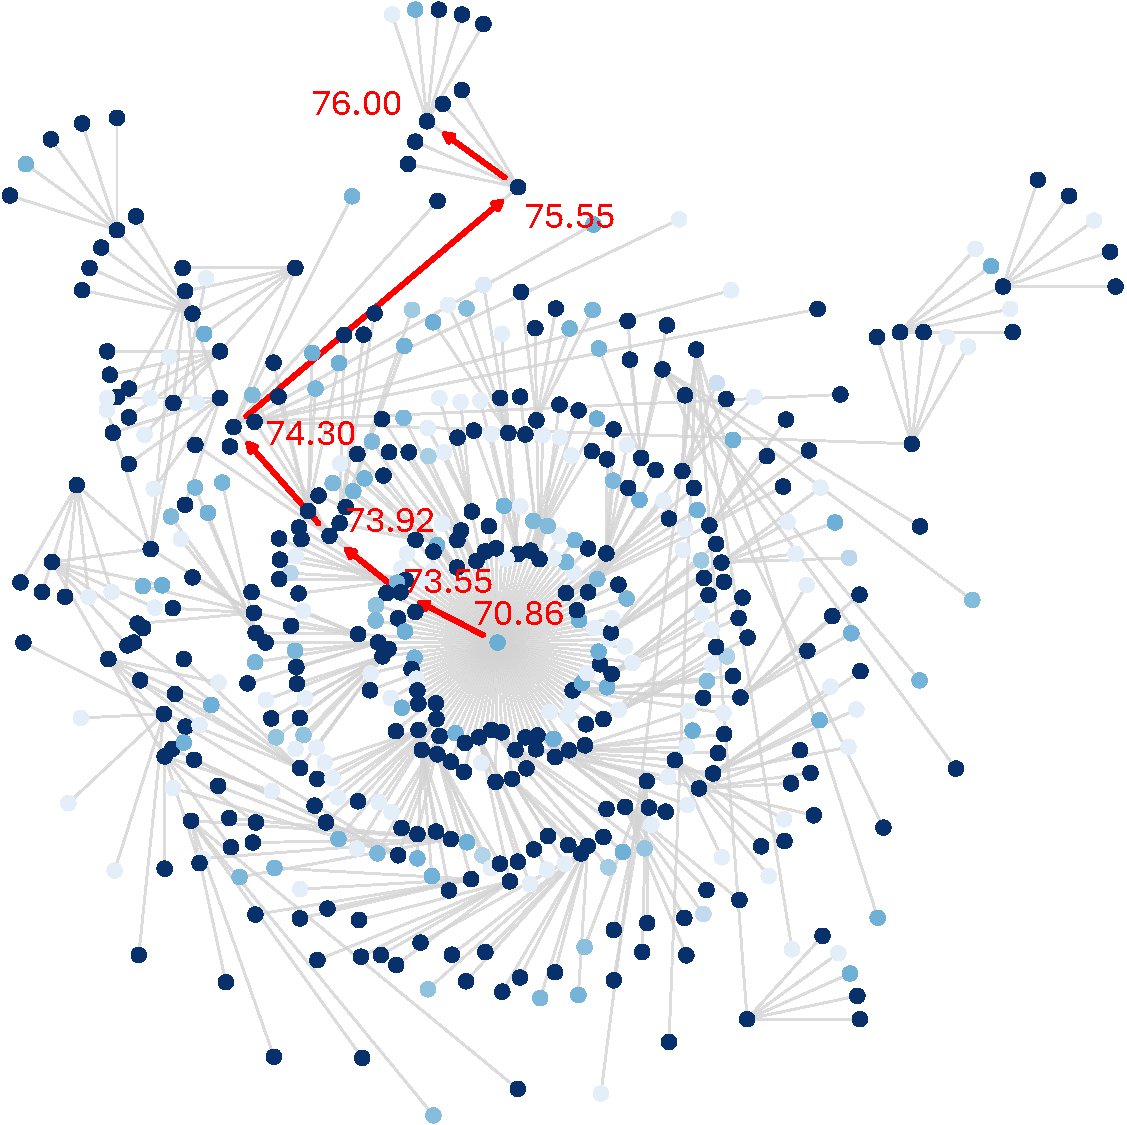
\includegraphics[width=0.8\linewidth]{figures/cifar100_run100.pdf}
    \caption{Large-scale NAD experiments.
    Each node represents a model, and the edge indicates which model is modified based on. The darker the node color, the higher the accuracy on the test set. 
    The root node in the center is ResNet.
    The path highlighted by the red arrows is the improvement path of the optimal model found.}
    \label{fig:large-scale}
\end{figure}
To further explore the potential of NADER, we use NADER to conduct a larger-scale neural architecture design on CIFAR100.
We initialize with ResNet~\cite{he2016deep} and generate 500 novel architectures using NADER. 
The modification process of these 500 architectures is shown in Figure~\ref{fig:large-scale}. 
To obtain these 500 architectures, we used 5,371K input tokens and 987K output tokens, totaling \$23 (\$2.50 per 1M input tokens and \$10.00 per 1M output tokens), resulting in an average cost of \$0.046 per architecture.
Finally, we get a novel architecture with an accuracy of 76.0\% on the test dataset, which is 5.14\% higher than the initial architecture. Futhermore, we evalute this architecture on the CIFAR-10 and ImageNet16-120. The experimental results, shown in Table ~\ref{tab:nasbench}, demonstrate that the designed architecture achieves strong performance across different datasets.